\documentclass[11pt]{article}

\usepackage{sectsty}
\usepackage{graphicx}
\usepackage{titlepic}
\usepackage{amsmath}

% Margins
\topmargin=-0.45in
\evensidemargin=0in
\oddsidemargin=0in
\textwidth=6.5in
\textheight=9.0in
\headsep=0.25in

\title{ EEM076 Lab1 \\
    \vspace{10}
    \large{Group Number 16}}
\author{ Albin Boklund, Samuel Runmark Thunell }
\date{\today}

\pagenumbering{gobble}

\begin{document}
\maketitle


\includegraphics[width = \linewidth]{lab1eem076frontpage.png}
\pagebreak

%--TASK1--

\section{\bf{Measuring currents}}

\subsection[25pt]{\bf{Calculations}}

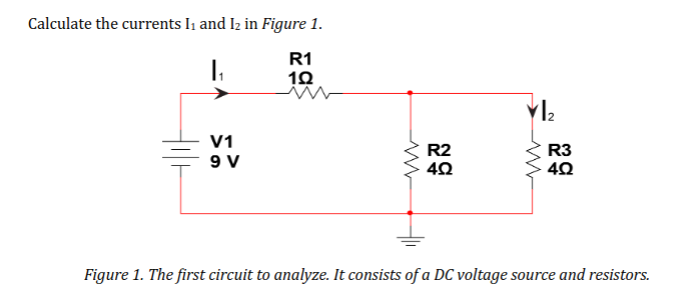
\includegraphics[width=\linewidth]{1.1 calculation.png}


\noindent
The value of $I_{1}$ can be calculated using $V = I*R$. This gives us $I_{1} = \frac{V1}{R1} = \frac{9V}{3\Omega} = 3A$. 
Since the circuit is parallel the current will be distributed accordingly to the difference between R2 and R3.
Since the difference is 0 the current will be divided equally (KCL). Giving us $I_{2} = \frac{3A}{2} = 1.5 A$



\subsection[25pt]{\bf{Circuit design and Simulation}}

\noindent
\\
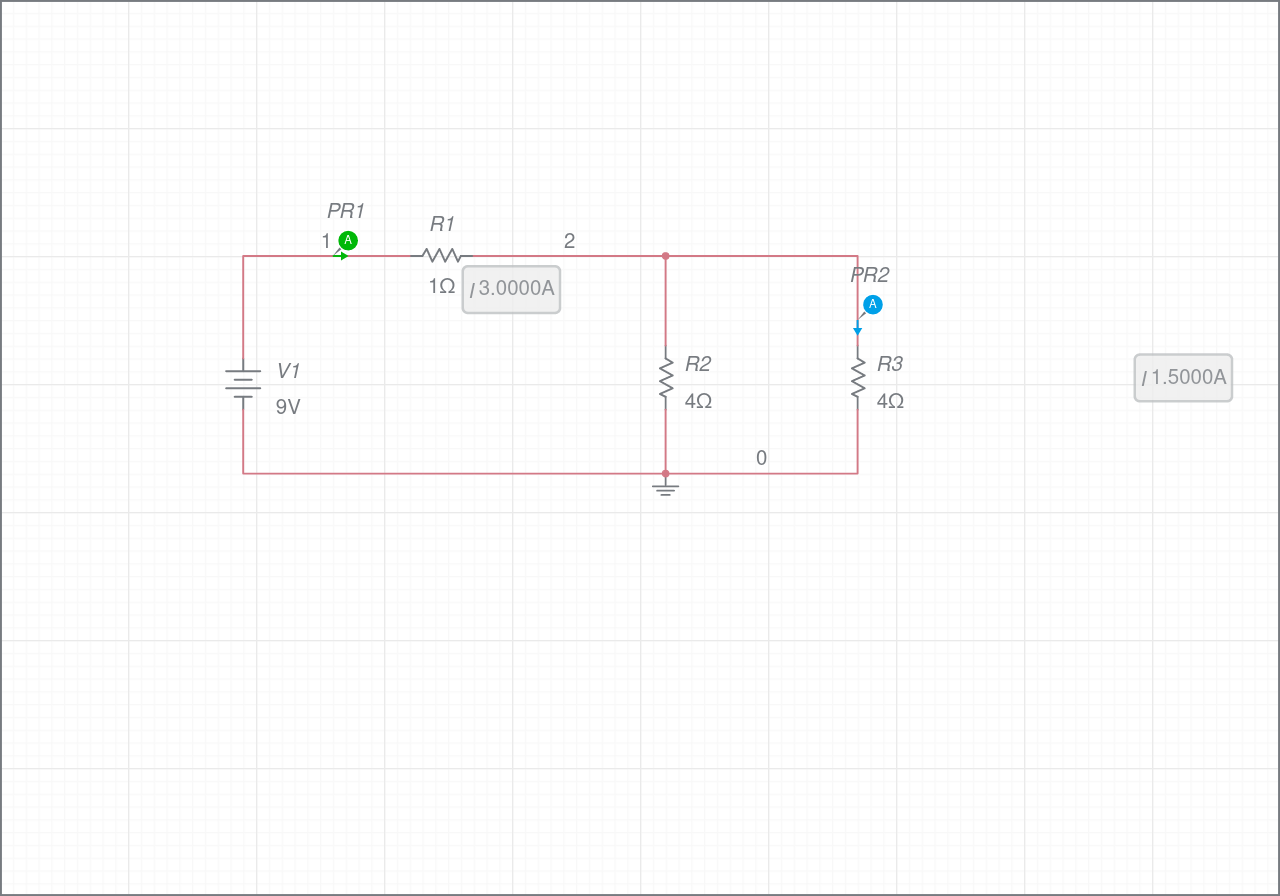
\includegraphics[width=\linewidth]{circuits/Lab 1 Task 1-schematic.png}


%--TASK2--
\section{\bf{Mesh analasys}}

\subsection[25pt]{\bf{Calculations}}

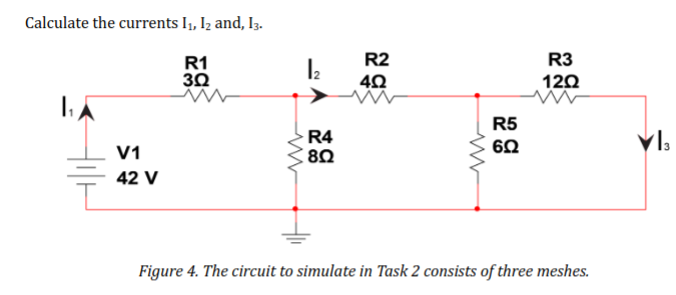
\includegraphics[width=\linewidth]{2.1 calculations.png}


\noindent
We first simplified the circuit using resistor equivalence for parallel resistors and then also for serial resistors.
This gives us $R235 = 8\Omega$. We know that the voltage will be $0$ at the ground and using this information and KCL we 
get the following equation $42V = 3I_{1} + 8(\frac{I_{1}}{2}) => 42 = 7I_{1} => I_{1} = \frac{42}{7} = 6A$.

\noindent
\\
Using $I_{1} = 6A$ we can use KCL to calculate $I_{2} = 3A$ and $I_{3} = 1A$.  

\subsection[25pt]{\bf{Circuit design and Simulation}}

\noindent
\\
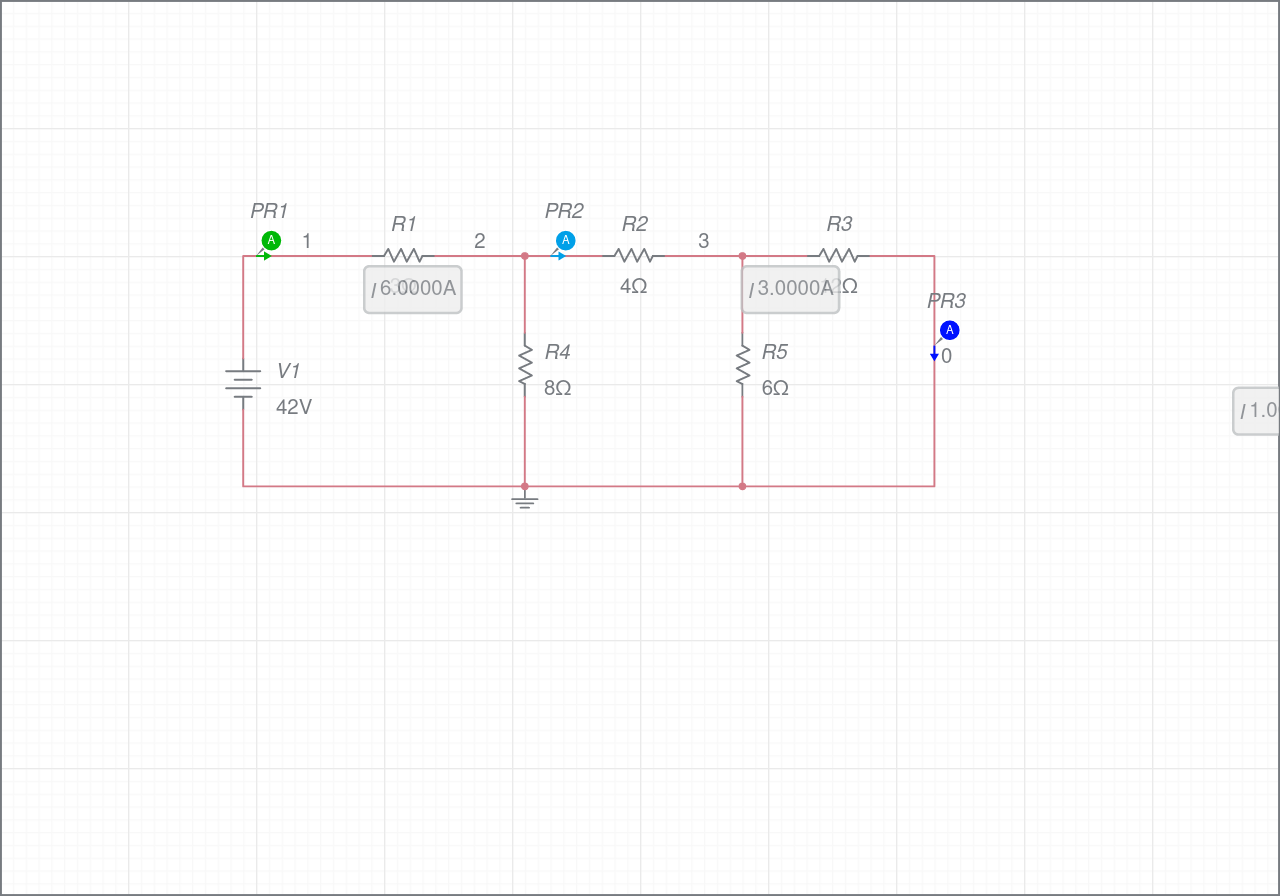
\includegraphics[width=\linewidth]{circuits/Lab 1 Task 2-schematic.png}


%--TASK3--
\section{\bf{The Superposition Principle}}

\subsection[25pt]{\bf{Calculations}}

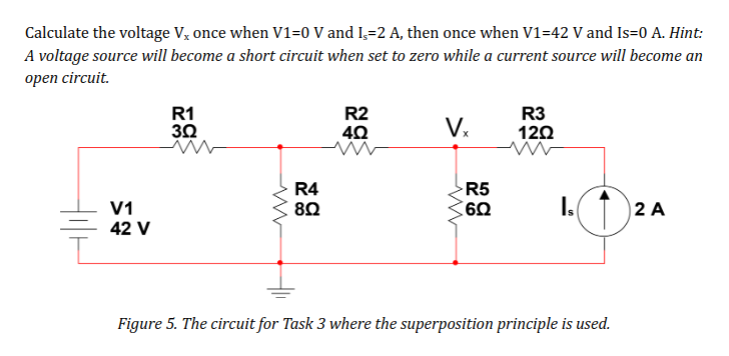
\includegraphics[width=\linewidth]{3.1 calculations.png}


\noindent
In the open circuit we can remove $R3$ from the circuit. We then calculate the serial resistor equivalence of $R2$ and $R5$
which gives us $R25 = 10\Omega$. We then use parallel resistor equivalence between $R4$ and $R25$ which equals $R425 = \frac{40}{9} \Omega$ 
Using this resistor we can then calculate the voltage between $R1$ and $R425$ using voltage divider (we call this voltage $V2$): 
$V2 = \frac{\frac{40}{9}}{\frac{40}{9} + 3} * 42 = \frac{1680}{67}V$. We can then return one step in the simplification
and then use the same tactic to calculate 
\\
$V_{x} = \frac{R5}{R2 + R5} * V2 = \frac{6}{4 + 6} * \frac{1680}{67} \approx 15.04V$

\noindent
\\
In the short circuit we use parallel resistor equivalence between $R1$ and $R4$, then serial resistor equivalence of $R14$ and $R2$ and then another 
parallel resistor equivalence between $R142$ and $R5$ which results $R1425 = \frac{204}{67}\Omega$. The highest voltage of the circuit can then be
 calculated to $V_{tot} = 2A * (12 + \frac{204}{67})$ Using voltage divider we can get $V_{x} = \frac{R1425}{R3 + R1425} * V_{tot} = 
 \frac{\frac{204}{67}}{12 + \frac{204}{67}} * 2 * (12 + \frac{204}{67}) = 6.08955$


\noindent
\\
To get the correct $V_{x}$ we add $V_{x_ Open circuit}$ and $V_{x_ Short circuit}$ which gives $15.04 + 6.08955 = 21.12955V$
 
\subsection[25pt]{\bf{Circuit design and Simulation}}

\noindent
\\
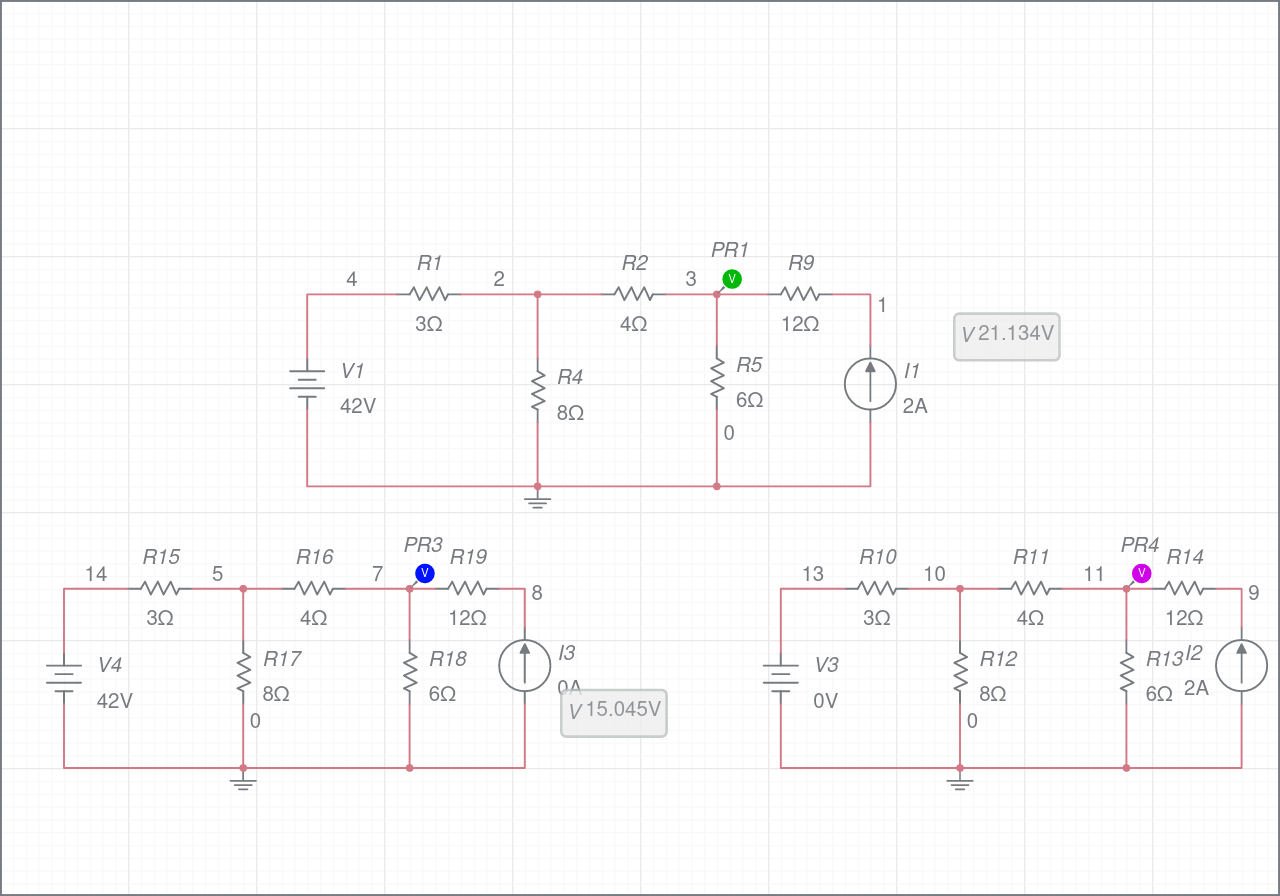
\includegraphics[width=\linewidth]{circuits/Lab 1 Task 3-schematic.png}

%--TASK4--
\section{\bf{Input and Output impedance}}

\subsection[25pt]{\bf{Calculations}}

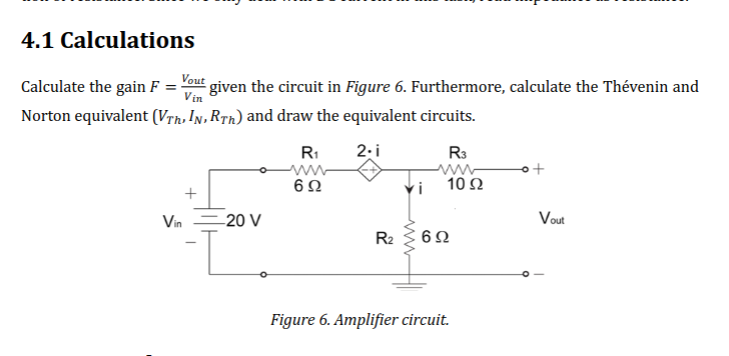
\includegraphics[width=\linewidth]{4.1 calculations.png}


\noindent
To start calculating the output voltage, we first need to calculate the current $i$ if we want to count or dependent source.
We start by rewriting the circuit as an open circuit, that means that we are left with only a loop, with $V_{in}$, $R_{1}$, $R_{2}$ and the dependent source.
Then we use KVL to calculate $i \Rightarrow R_{1}*i - 2i + R_{2}*i = 20$.
Which leaves us with $i = 2$.
We can now calculate $V_{out} = i*R_{2} = 2A*6\Omega = 12V$.
The gain of the circuit is therefore $F = \frac{V_{out}}{V_{in}} = \frac{12}{20} = 0.6$.
\noindent
\\

\noindent
To calculate the Thévenin and Norton equivalent circuits we can start by rewriting it as a closed circuit.
We can now define the currents over the resistors with their corresponding numbering.
Using KVL on both loops and KCL at the junction right after the dependent source, we get three equations:

\begin{gather*}
    \begin{cases}
        -V_{in} + R_{i}*i_{1}-2*i_{2} + R_{3}*i_{3} = 0 \\
        R_{3}*i_{3} = R_{2}*i_{2} \\
        i_{1} = i_{2} + i_{3}
    \end{cases}
\end{gather*}

\noindent
Solving for $i_{3}$, we get $i_{3} = \frac{15}{17}$ which is also our Norton current $i_{N}$.

\noindent
We can now calculate $R_{th}$ using $V_{th} = V_{out}$ and $i_{N}$. \\
$R_{th} = \frac{V_{th}}{i_{N}} = \frac{12}{\frac{15}{17}} = \frac{68}{5}$

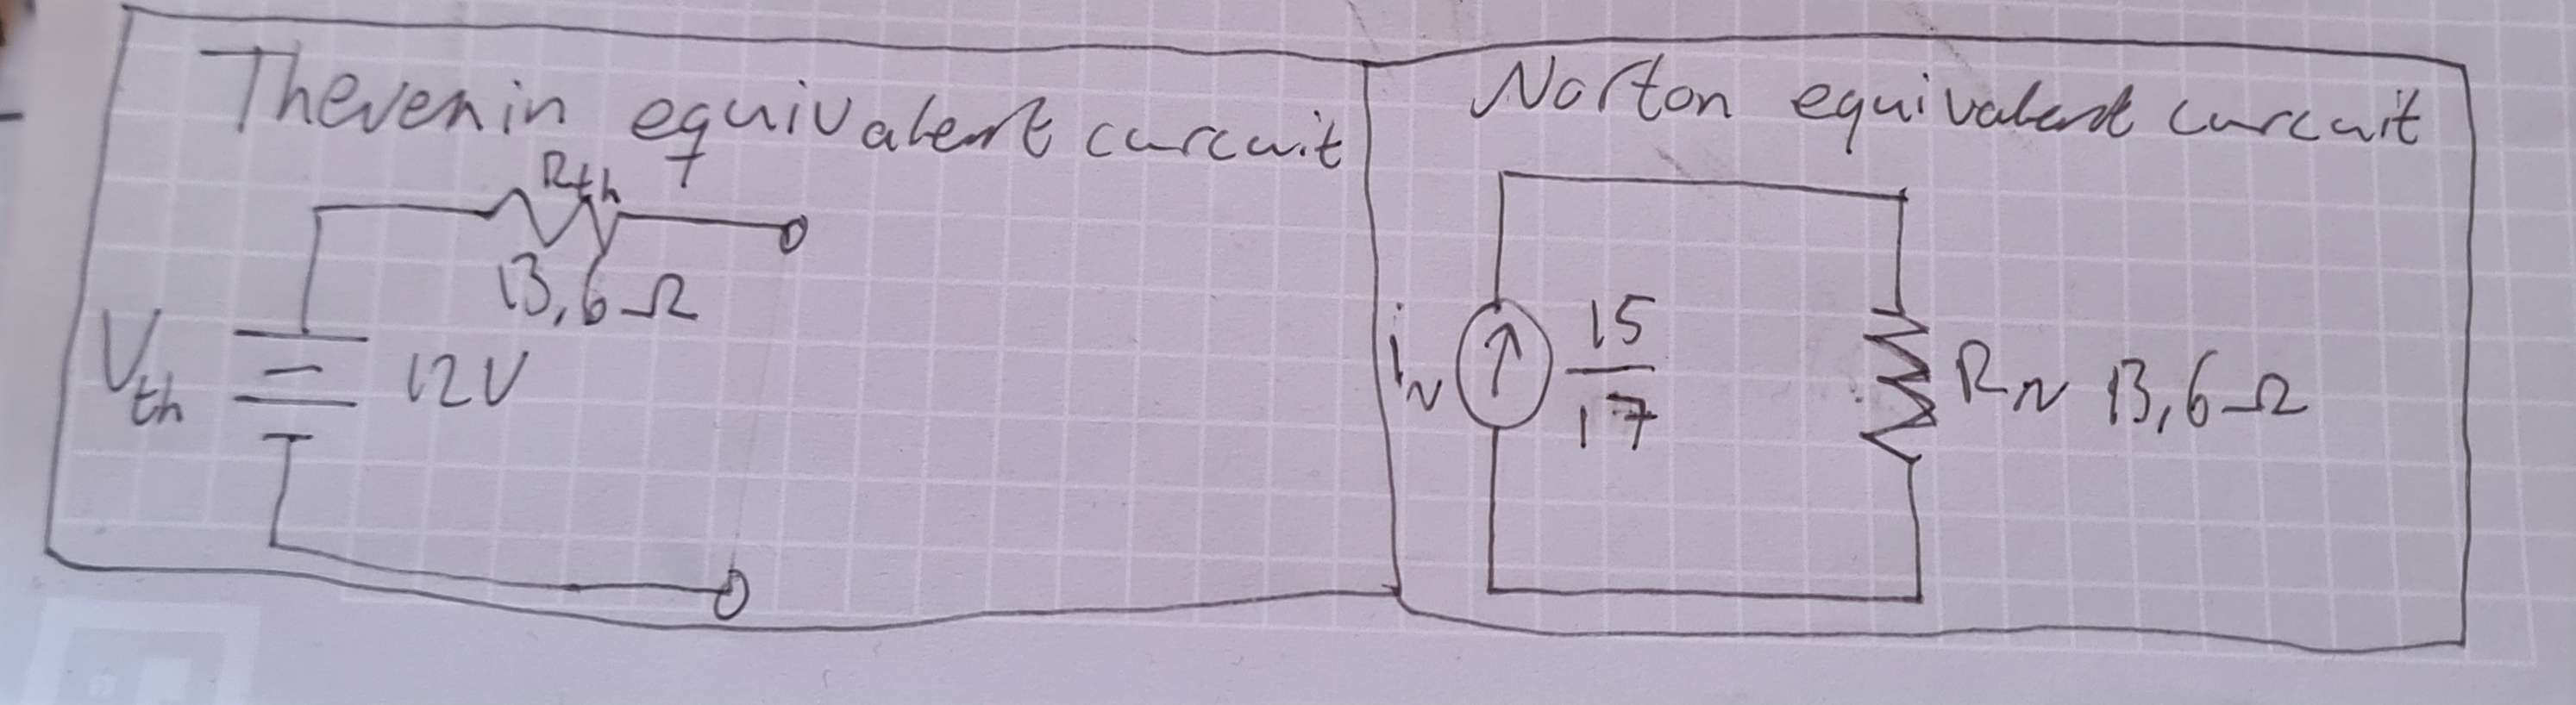
\includegraphics[width=\linewidth]{4.1curcuits.jpg}

\subsection[25pt]{\bf{Circuit design and Simulation}}

\noindent
\\
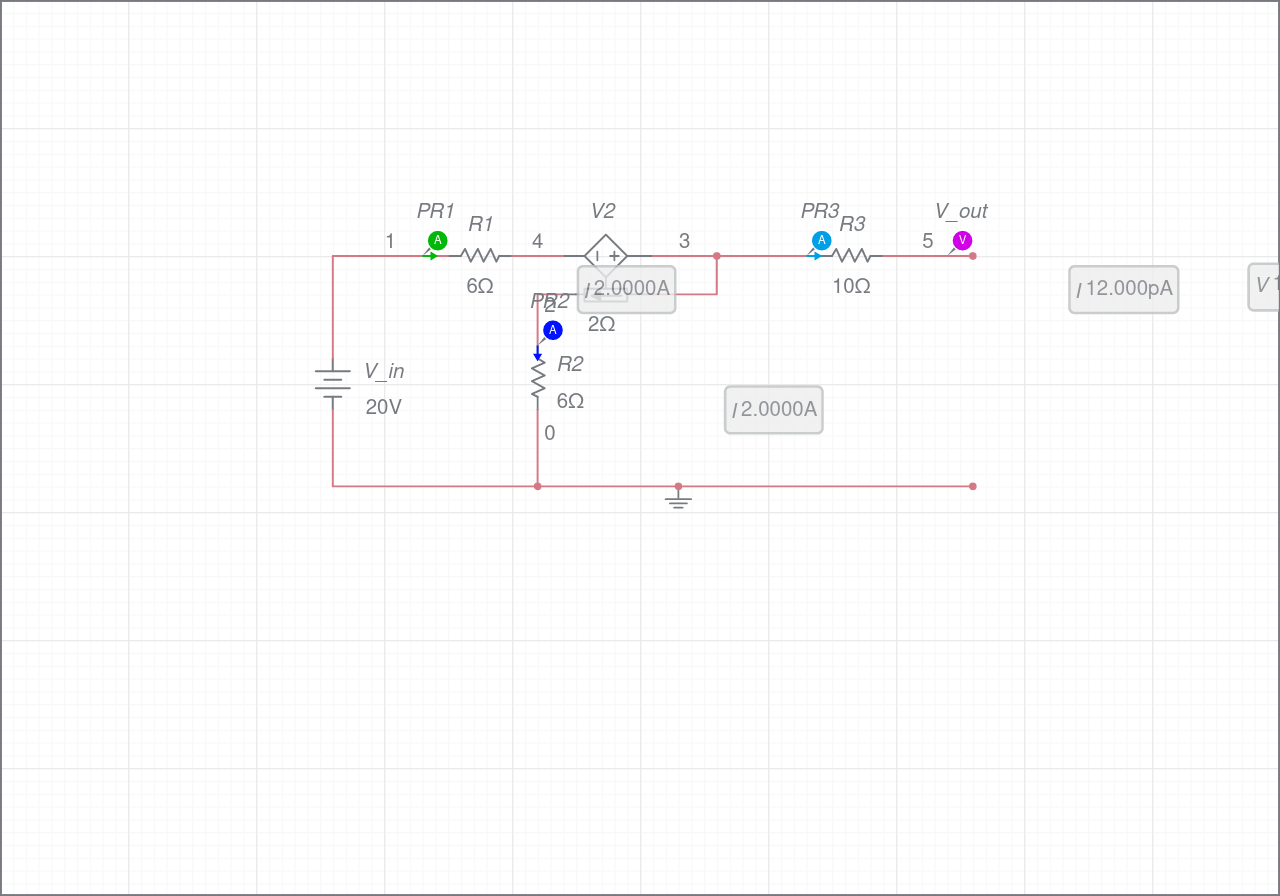
\includegraphics[width=0.5\linewidth]{circuits/Lab 1 Task 4-schematic.png}
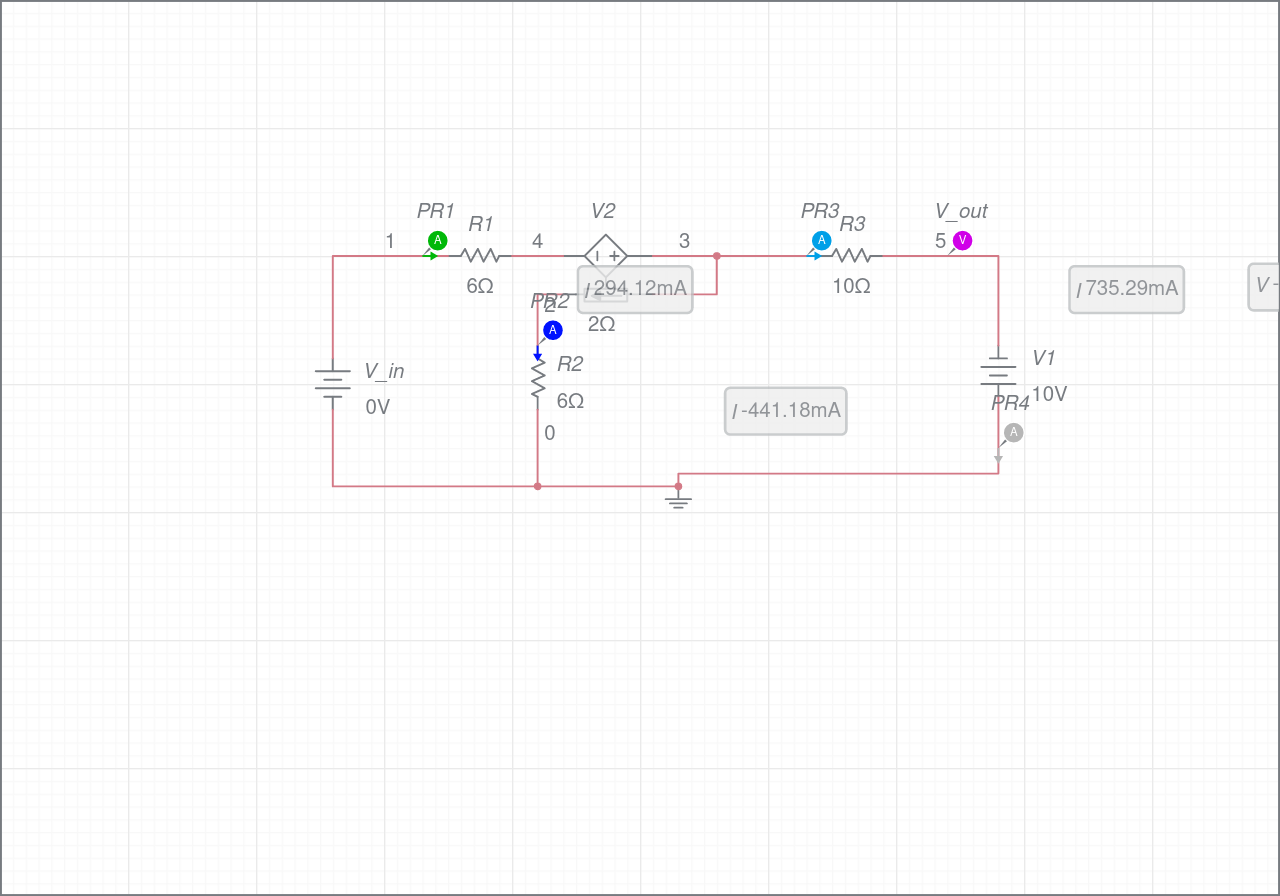
\includegraphics[width=0.5\linewidth]{circuits/Lab 1 Task 4-schematic(2).png}
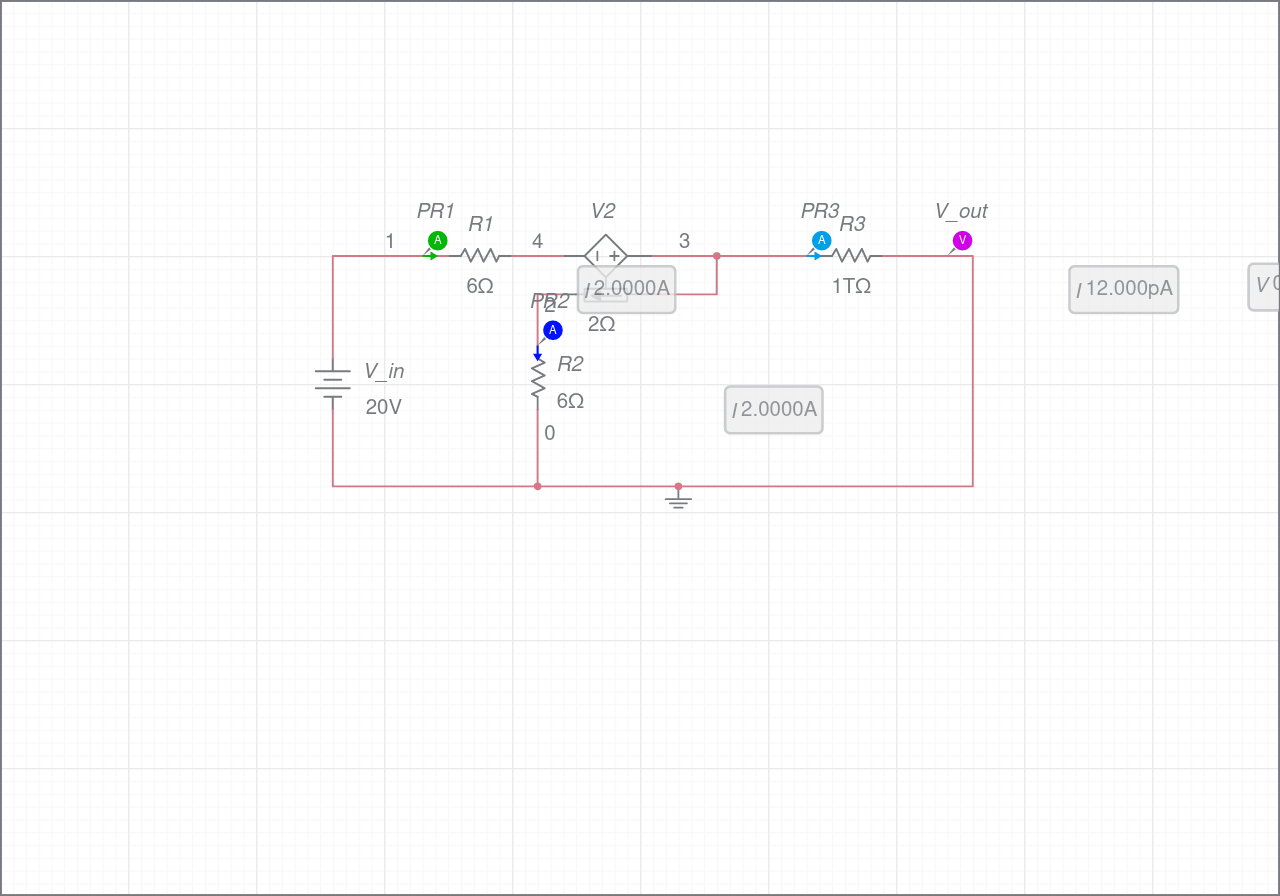
\includegraphics[width=0.5\linewidth]{circuits/Lab 1 Task 4-schematic(1).png}
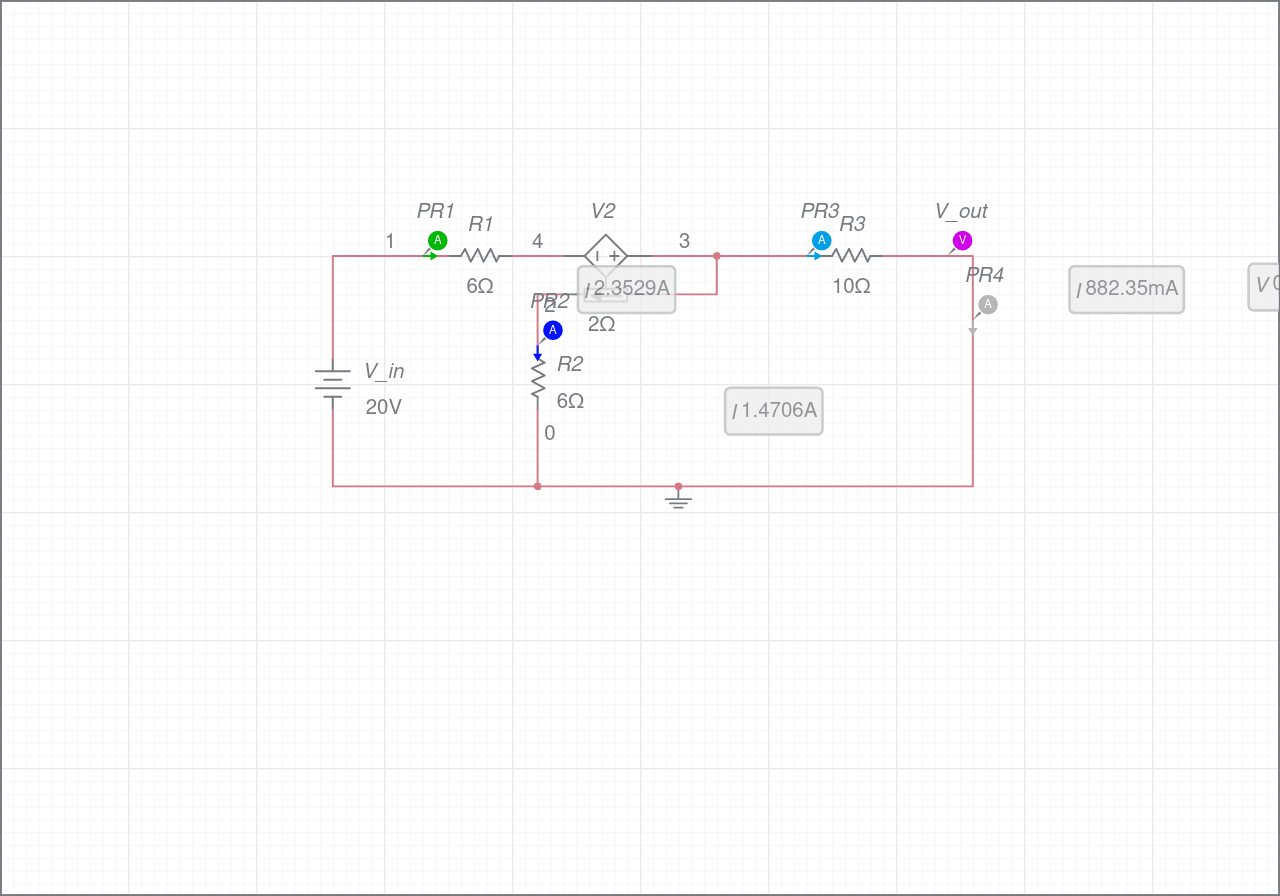
\includegraphics[width=0.5\linewidth]{circuits/Lab 1 Task 4-schematic(3).png}


%--TASK5--
\section{\bf{Maximal power from a voltage source}}

\subsection[25pt]{\bf{Calculations}}

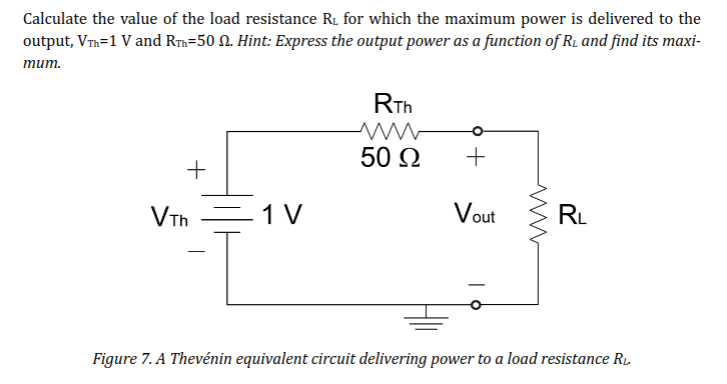
\includegraphics[width=\linewidth]{5.1 calculations.png}


\noindent
To get the Power (P) we use the formula $P = i² * R$. We want to calculate the power over $R_{L}$  so we use $R_{L}$ as R.
 This gives us $(\frac{1}{50 + R_{L}})^2 * R_{L} = \frac{R_{L}}{(50 + R_{L})^2}$. Simulating this in GeoGebra we get that the maximum power is $0.01W$ at
 $R_{L} = 50\Omega$. This is also supported by the maximum power theorem. 

\subsection[25pt]{\bf{Circuit design and Simulation}}

\noindent
\\
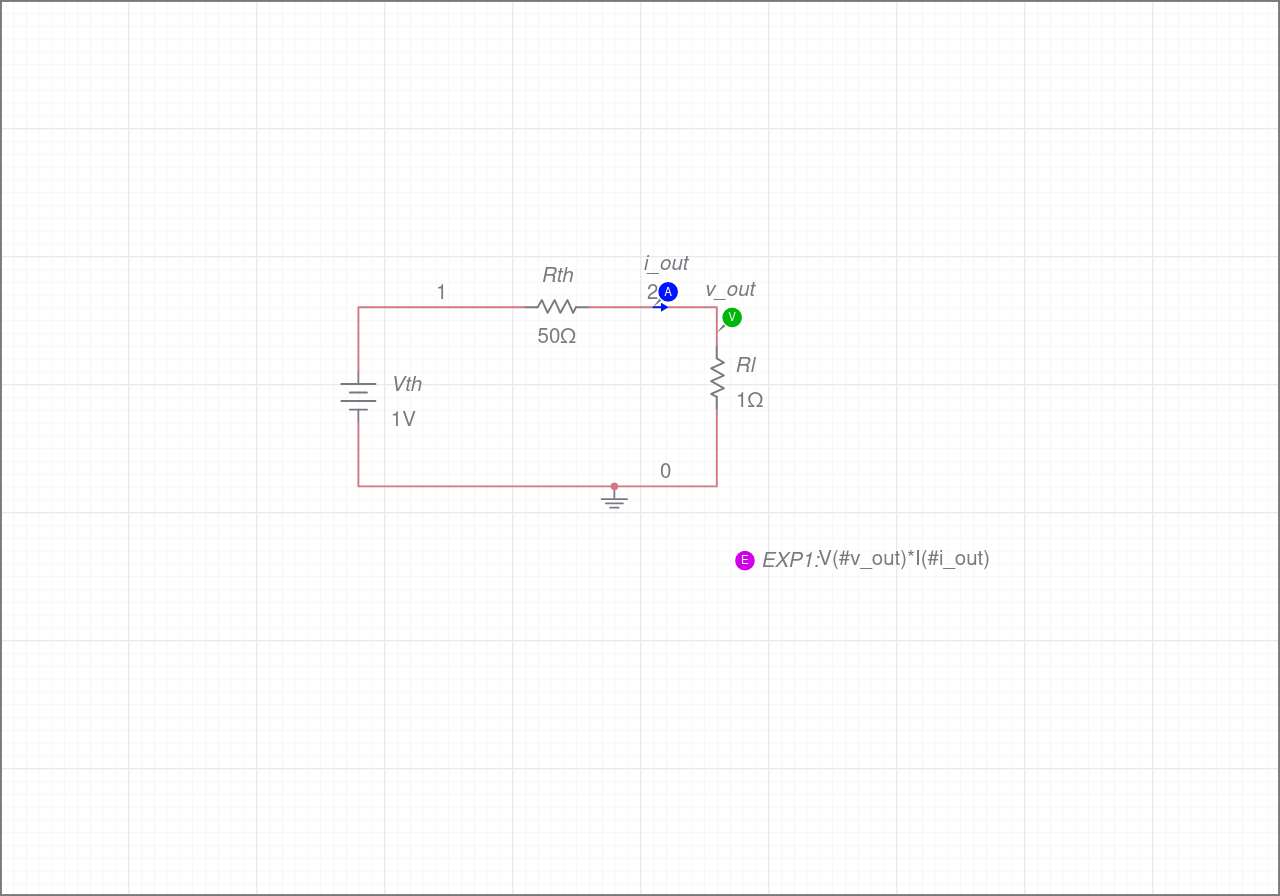
\includegraphics[width=\linewidth]{circuits/Lab 1 Task 5-schematic.png}

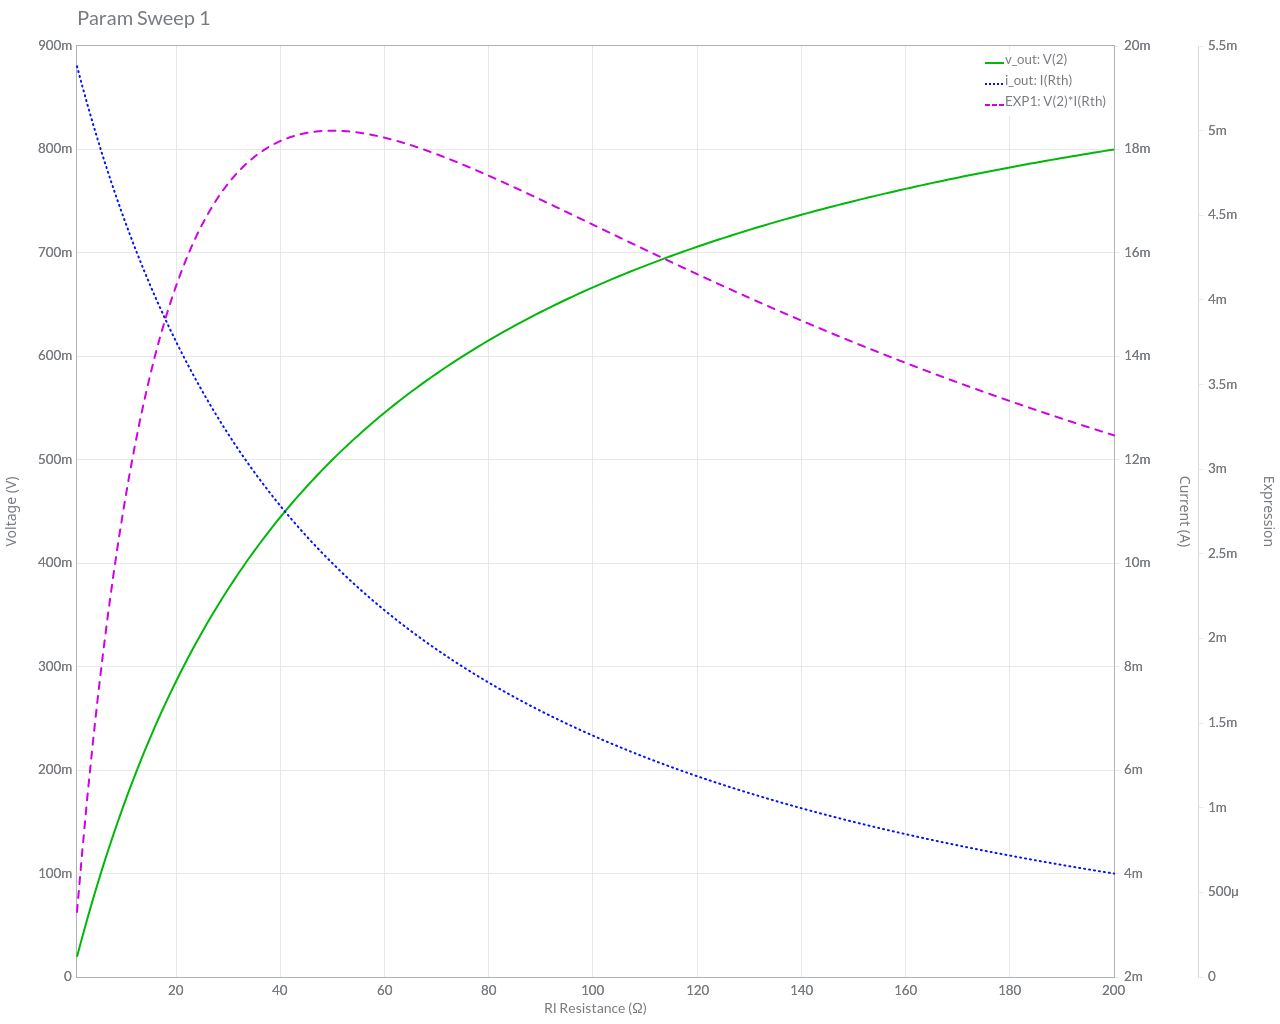
\includegraphics[width=\linewidth]{circuits/Lab 1 Task 5-Grapher.png}

%--TASK6--
\section{\bf{Maximum power from a current source}}

\subsection[25pt]{\bf{Calculations}}

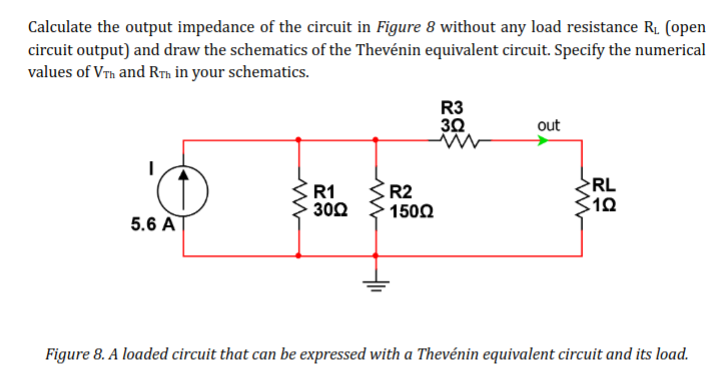
\includegraphics[width=\linewidth]{6.1 calculations.png}

\noindent
We started by calculating the Norton and Thévenin equivalent circuits of the given circuit. 
The first step was to calculate the Thévenin resistance by rewriting it as an open circuit by opening both the load resistance and the current source.
We continue by combining the resistances into one equivalent. This turned out to be a single resistor with $28\Omega$.
This means that $R_{th} = 28\Omega$.

\noindent
\\
The next step was to short the circuit to calculate the Thévenin voltage. We combine the two parallel resistors by $frac{30\Omega * 150\Omega}{30\Omega + 150\Omega = 25\Omega}$
The Thévenin voltage is therefore calculated by: $V_{th} = I * R = 5.6 * 25 = 140V$.

\noindent
\\
$R_{N} = 28\Omega$
\noindent
\\
$I_{N} = 5.6A$
\noindent
\\
$R_{th} = 28\Omega$
\noindent
\\
$V_{th} = 140V$

\subsection[25pt]{\bf{Circuit design and Simulation}}

\noindent
\\
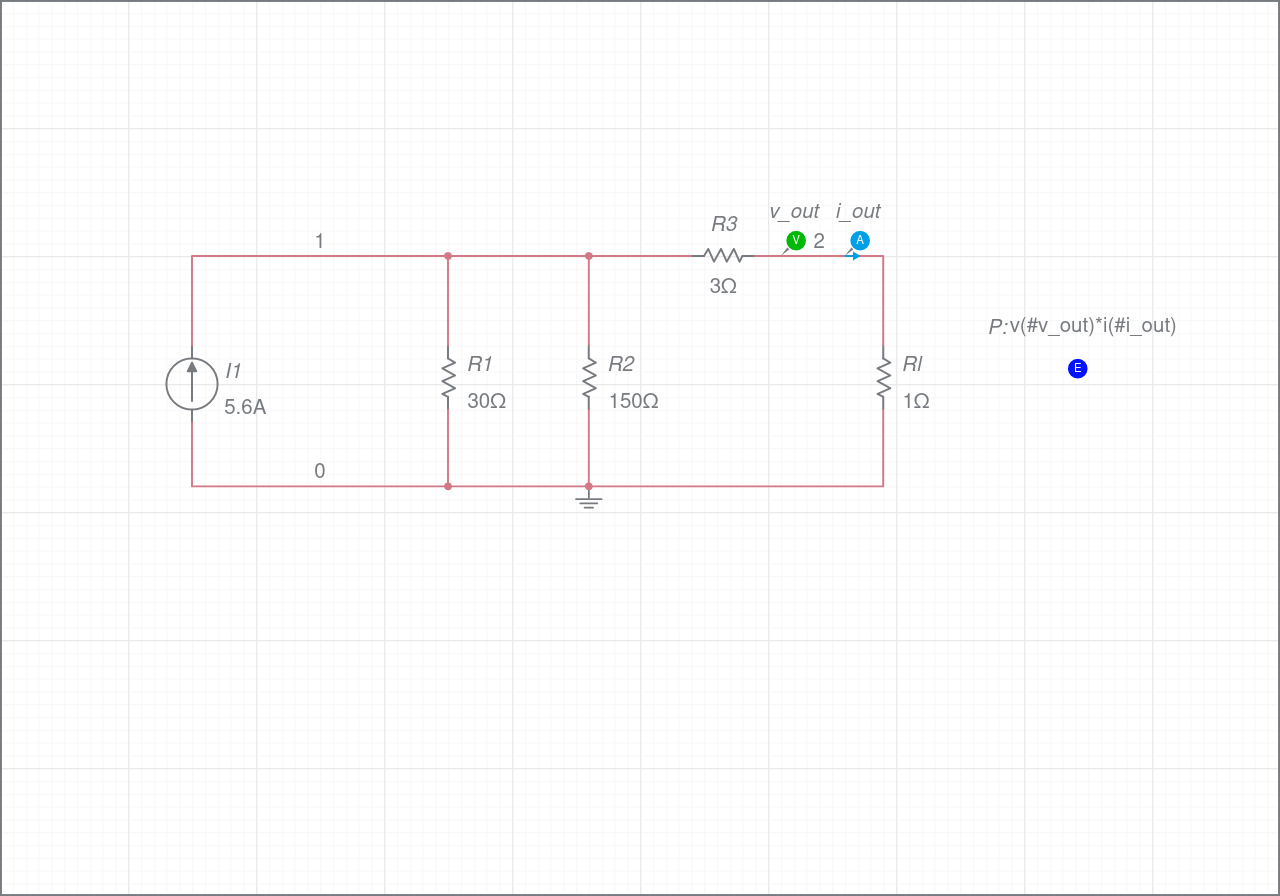
\includegraphics[width=\linewidth]{circuits/Lab 1 Task 6-schematic.png}

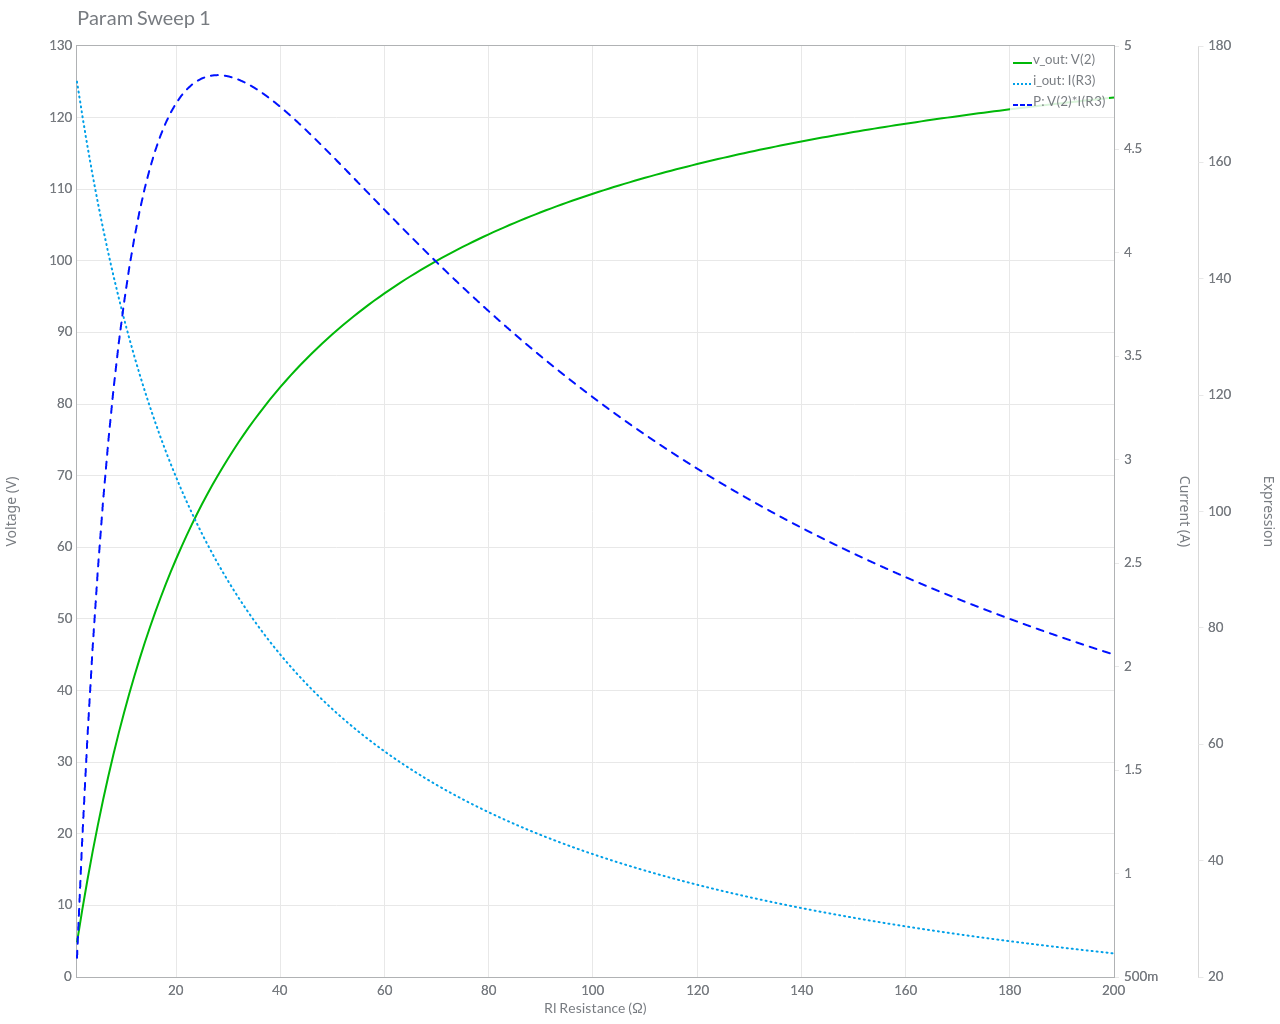
\includegraphics[width=\linewidth]{circuits/Lab 1 Task 6-Grapher.png}

\noindent
\\
Our calculations are supported by the simulation, we can see that we attain our max power at $R_{L} = 28\Omega$. Which we also calculated before.

\end{document}